\appendix

\section{Приложение A: Техническая документация INR-21700-P42A}\label{app:INR21700}
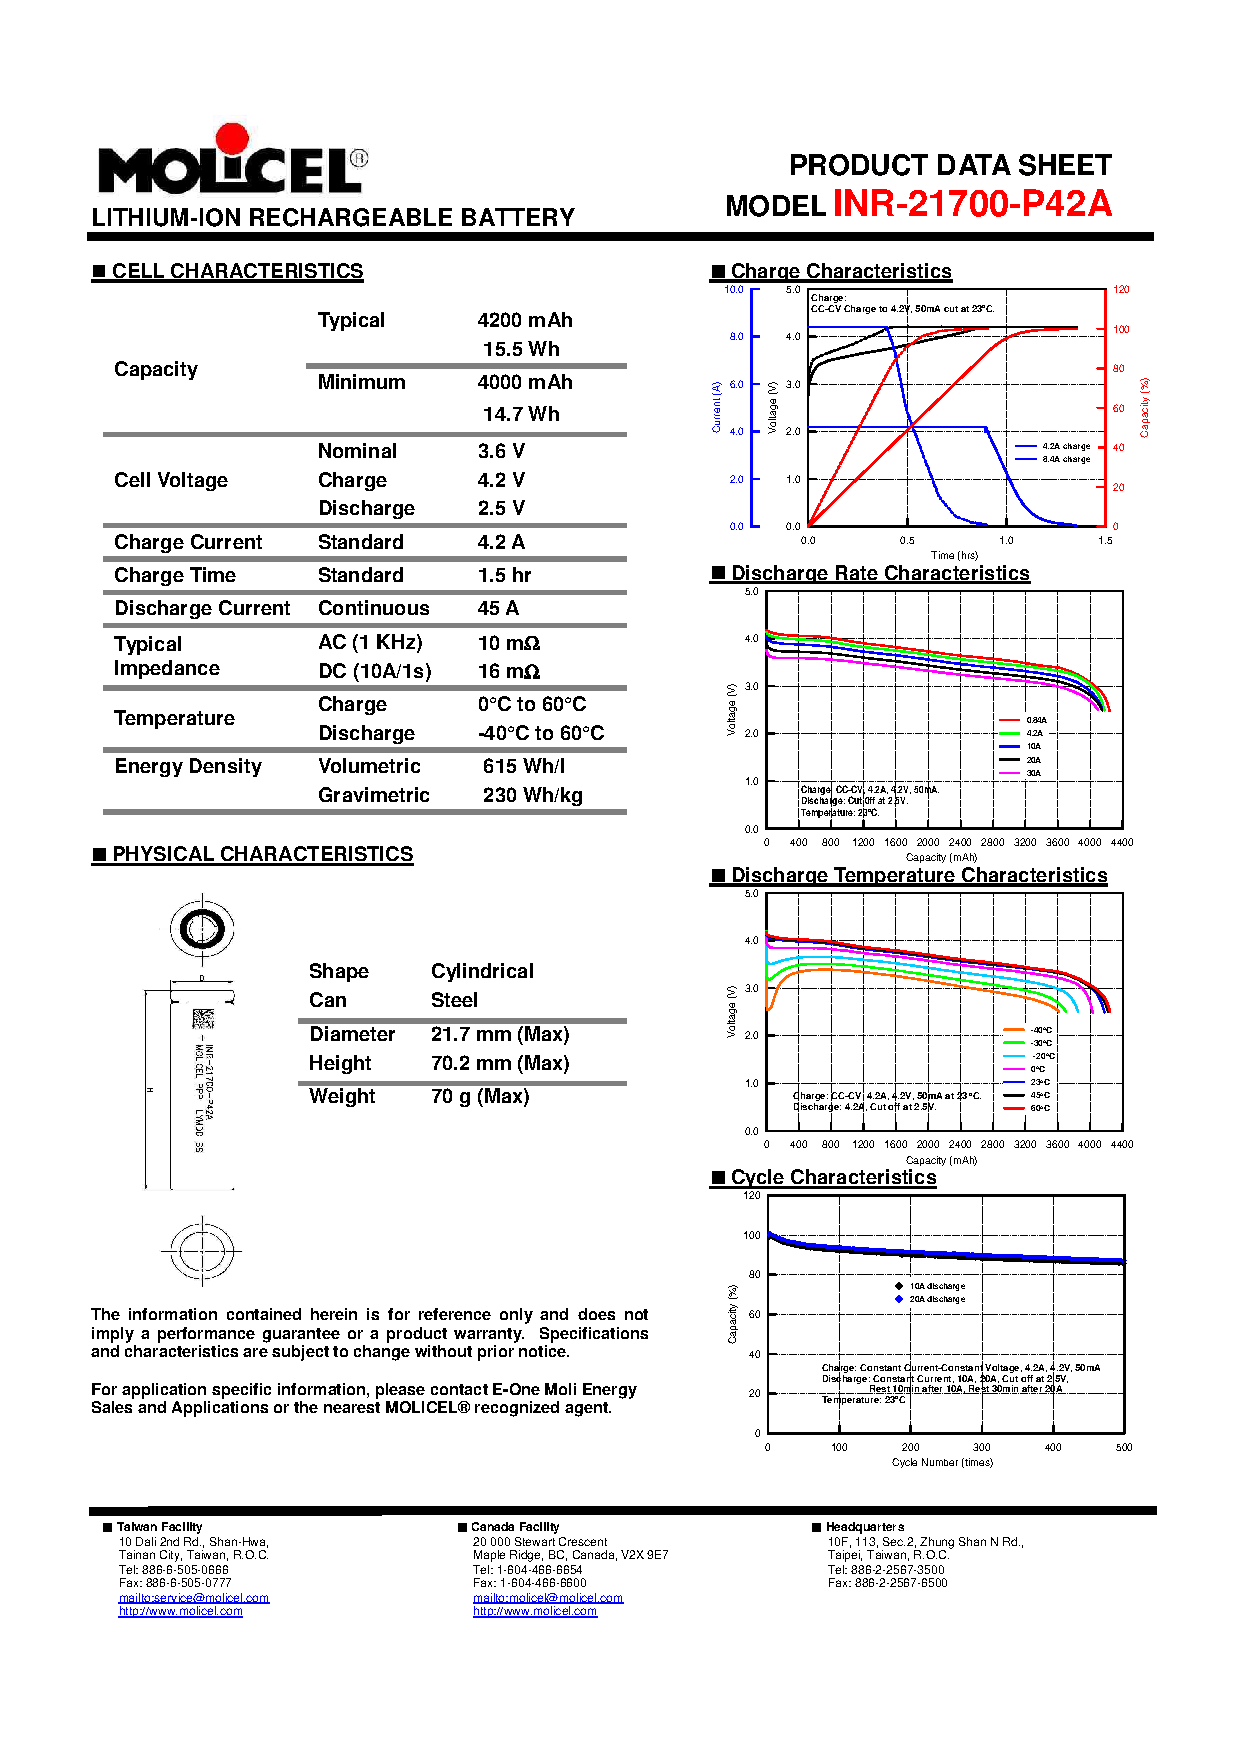
\includepdf[pages=-, scale=0.95]{applications/INR21700P42A-V3-80092.pdf} % Вставляет все страницы PDF

\section{Приложение B: Кривые характеристик микросхемы TL-431}\label{app:TL431_CURVES}
\includepdf[pages=3, scale=0.95]{applications/TL_431_datasheet.pdf}

\section{Приложение C: Симуляция балансировочной схемы}\label{app:falstad}
Для симуляции был использован расчётчик от Paul Falstad. \\
Интерактивная ссылка на схему \href{https://falstad.com/circuit/circuitjs.html?ctz=CQAgjCAMB0l3BWEDoBYEE4AcYFwMz5iqoBMqIqAbMspMgKYC0YYAUAO7gJYWlZZwAdjCkQ-QZDYBnYaPEDhGMRKhqAZgEMANtIaduvcP3BUs9UZLYAncBjOUwNMPcGW1T6FgNPzyE2C89AgmUraBqPSo+GIRwaHg8FJcvvQxFmYWoT6ZlDGmfpH0YQVppBmFcGpY5cngQcZuue51ceJCsQ0tPg34kBRt0Sps6nb9ebGuEyD5+OL40Ahs+QA6xeCwSVtbYMxOahaLB+Lgp+vsAC5KKoptqvQsM9BUpEJCGH2ouKJUVBRMMEgpAwYEg9iBkFwVEgVD6ziqaxy+yGpWmpBsqJRg3y9FItTgGNS-iahRxxngPh4FBCJPiVhSVOJ4HQNBpUDYXwsCBClCqxAQrICQKQAD8ACoAGWiEEgK2kkRAVDluxYpDlMA6qHeuHIpF+Wo+6vVirlpD2aukLEW5Rw+CEqBB1H6ISN0mKyrlVpCkFt9sd0PQFo15G1ITI+ve+GVkTlIou2mlDAAJkwAI4AOwA+smoHKYn5ZdJyFVCx0S3mFoQq9WazQldIwNAzar1dAhD6BDC+rxsJCg8b66Q0ObPYD4HisPgqKwtQLeKJ+27cw3R5s4BOpzOhHOvnjW+2BOZYT6HeZRNHC3GE0Rk2ms7eAIKNsSFwLQQIfnBfz8motN7YAZA+Ajm6zxCPgZAYAgRDlNKpBRm6A5yqgaCATsIGAn8rD4BgYKkC4yhYL8rruiuoEwl8YA4XhBH8MRoFUOBkHQaI-QwQhxCXvGiYphm2Ypg+Q4vnK5ikQq9YqueDEkFRBFYNgHxEKgJG-s2UlevY0FUCC2HEMoymIUur6eo2mBUFpOmyQ65Ctn8XxEBgCnyYQxAXrG3E3rx95JsuRRifQEkYc8JBCF+1moFgeBYCpg4gQC752l2ThmPBYBvIupFgKuVHtrCyU1EQ6W2SFYX6ZFPpudIV48Xe-HLn49YIHsCEwNpOAfCQWDgR8xAZb+klBmB8EQQK7bYNQPAqcZDEdIQLJjbw5nRQx2AuBBEXdUpFqce5167F5-FMA+MBIIWDXKnFrXRF1kV9H6CC4DFeZBVsRH4Jg5VEdC5D1oWpEsK2r2wh9UW-EC1Crn8+A3dBkD3Y90jQrtNWpgADnVZ0BRdLaWldU4dQgJARTgDpPdIwE4wsQIOaCuCKSQjFTSZeawKlIKQpgc3UEIkPRNpI1EwIelykjVUeftabozmmOkaJvlYw2L2kDwfTAvAdqsP0y1-apcULIxeIhO2yt4tQU5M2RTD6x0JvGyEP3m+RyuTkCuEECIoIRZV1WebV0vKng9W-k1ONjuub3oJELzTkBgZk5JWWWvrvY1BgIiE38sK-ca01W88KfAun1Bm79a5AhHhMwnqoIjdtMZi3tt58Y+p3Kkk8v9XFQ7fBFrERUBc084ZCtqRaVDPHDLzboEkAICIQLMBgFuJ+P0JCFPD3mHPoLNkvlrdw9veweYVZat74tN954jI77SYY23VQWj7Et3zmgUsIn1uG685AM+QCM61ih-bKiVpzKwFIQScrASKEkZKoXARgpySG4K0FkjRDADGyOEOBPoMEKGQTPHoCosS4QoCiKQqMxhkPyC4cYbI5jnAAj4KYbIXAOE6uyRKeD3AIL4LghhnD2z1AVDwqY7gBEUPEEBMQXwaDlHyPQ44oJthsAAErMgFOg3qmCCGJGKEcBYGADiLDYAAcw0YKNwaCBTrEkfyZwARrEmAkXorYlIjAOmcIyNkdR5EyP2GwwQsj2QpBYSYPxTJWgNFYaQyJzCHAxLodkAAHtwaCIBtx2GhhkoJ4gKCAEQQQADCCAG4QQpgBeEEAIIggAOEEAAIggA+EEAEwgdTADiIGUwpgB5EDlBUwAoiCAFYQQAPCCFLlIAFhBimdOkBKAAlkwSZAB7dMbBZkzAgH8NQyTabrloDAGU4BFl5JAMgyI2AtnvlOOwJZrxKBqCOUY06aATgqCEDMNgQA}{\color{blue}{тут}}.

Текстовая ссылка:\\
\seqsplit{https://falstad.com/circuit/circuitjs.html?ctz=CQAgjCAMB0l3BWEDoBYEE4AcYFwMz5iqoBMqIqAbMspMgKYC0YYAUAO7gJYWlZZwAdjCkQ-QZDYBnYaPEDhGMRKhqAZgEMANtIaduvcP3BUs9UZLYAncBjOUwNMPcGW1T6FgNPzyE2C89AgmUraBqPSo+GIRwaHg8FJcvvQxFmYWoT6ZlDGmfpH0YQVppBmFcGpY5cngQcZuue51ceJCsQ0tPg34kBRt0Sps6nb9ebGuEyD5+OL40Ahs+QA6xeCwSVtbYMxOahaLB+Lgp+vsAC5KKoptqvQsM9BUpEJCGH2ouKJUVBRMMEgpAwYEg9iBkFwVEgVD6ziqaxy+yGpWmpBsqJRg3y9FItTgGNS-iahRxxngPh4FBCJPiVhSVOJ4HQNBpUDYXwsCBClCqxAQrICQKQAD8ACoAGWiEEgK2kkRAVDluxYpDlMA6qHeuHIpF+Wo+6vVirlpD2aukLEW5Rw+CEqBB1H6ISN0mKyrlVpCkFt9sd0PQFo15G1ITI+ve+GVkTlIou2mlDAAJkwAI4AOwA+smoHKYn5ZdJyFVCx0S3mFoQq9WazQldIwNAzar1dAhD6BDC+rxsJCg8b66Q0ObPYD4HisPgqKwtQLeKJ+27cw3R5s4BOpzOhHOvnjW+2BOZYT6HeZRNHC3GE0Rk2ms7eAIKNsSFwLQQIfnBfz8motN7YAZA+Ajm6zxCPgZAYAgRDlNKpBRm6A5yqgaCATsIGAn8rD4BgYKkC4yhYL8rruiuoEwl8YA4XhBH8MRoFUOBkHQaI-QwQhxCXvGiYphm2Ypg+Q4vnK5ikQq9YqueDEkFRBFYNgHxEKgJG-s2UlevY0FUCC2HEMoymIUur6eo2mBUFpOmyQ65Ctn8XxEBgCnyYQxAXrG3E3rx95JsuRRifQEkYc8JBCF+1moFgeBYCpg4gQC752l2ThmPBYBvIupFgKuVHtrCyU1EQ6W2SFYX6ZFPpudIV48Xe-HLn49YIHsCEwNpOAfCQWDgR8xAZb+klBmB8EQQK7bYNQPAqcZDEdIQLJjbw5nRQx2AuBBEXdUpFqce5167F5-FMA+MBIIWDXKnFrXRF1kV9H6CC4DFeZBVsRH4Jg5VEdC5D1oWpEsK2r2wh9UW-EC1Crn8+A3dBkD3Y90jQrtNWpgADnVZ0BRdLaWldU4dQgJARTgDpPdIwE4wsQIOaCuCKSQjFTSZeawKlIKQpgc3UEIkPRNpI1EwIelykjVUeftabozmmOkaJvlYw2L2kDwfTAvAdqsP0y1-apcULIxeIhO2yt4tQU5M2RTD6x0JvGyEP3m+RyuTkCuEECIoIRZV1WebV0vKng9W-k1ONjuub3oJELzTkBgZk5JWWWvrvY1BgIiE38sK-ca01W88KfAun1Bm79a5AhHhMwnqoIjdtMZi3tt58Y+p3Kkk8v9XFQ7fBFrERUBc084ZCtqRaVDPHDLzboEkAICIQLMBgFuJ+P0JCFPD3mHPoLNkvlrdw9veweYVZat74tN954jI77SYY23VQWj7Et3zmgUsIn1uG685AM+QCM61ih-bKiVpzKwFIQScrASKEkZKoXARgpySG4K0FkjRDADGyOEOBPoMEKGQTPHoCosS4QoCiKQqMxhkPyC4cYbI5jnAAj4KYbIXAOE6uyRKeD3AIL4LghhnD2z1AVDwqY7gBEUPEEBMQXwaDlHyPQ44oJthsAAErMgFOg3qmCCGJGKEcBYGADiLDYAAcw0YKNwaCBTrEkfyZwARrEmAkXorYlIjAOmcIyNkdR5EyP2GwwQsj2QpBYSYPxTJWgNFYaQyJzCHAxLodkAAHtwaCIBtx2GhhkoJ4gKCAEQQQADCCAG4QQpgBeEEAIIggAOEEAAIggA+EEAEwgdTADiIGUwpgB5EDlBUwAoiCAFYQQAPCCFLlIAFhBimdOkBKAAlkwSZAB7dMbBZkzAgH8NQyTabrloDAGU4BFl5JAMgyI2AtnvlOOwJZrxKBqCOUY06aATgqCEDMNgQA}

% Ниже представлена схема в текстовом виде в формате расчётчика.
% \begingroup
%     \fontsize{9pt}{12pt}\selectfont
%     \begin{verbatim}
%         $ 1 0.000005 5.459815003314424 46 5 50 5e-11
%         w 1584 288 1712 288 0
%         s 1712 288 1792 288 0 0 false
%         w 1584 128 1680 128 0
%         r 1968 416 1968 128 0 16.8
%         w 1680 528 1840 528 0
%         r 1840 432 1840 528 0 10000
%         w 1680 320 1680 128 0
%         w 1680 432 1680 400 0
%         r 1680 320 1680 400 0 8200
%         w 1840 128 1680 128 0
%         w 1840 272 1840 128 0
%         w 1840 304 1840 432 2
%         f 1904 432 1968 432 32 3 23.5
%         32 \0 0 1.0000000000000001e-16 0 0 1.5 0 0 2 1 1 0 0 1
%         t 1792 288 1840 288 0 -1 -0.8205670736596202 -0.8394308153525953 100 \0
%         w 1616 432 1680 432 2
%         r 1680 432 1840 432 0 220000
%         r 1680 528 1680 432 0 12000
%         w 1584 528 1680 528 0
%         w 1584 528 1456 528 0
%         410 1552 400 1456 528 1025 ~TL431 0\s40 6\s1e-12\s0.7392237234888934\s0\s0 6\s2e-12\s0.6605168925865894\s0\s0 0\s1\s0.6605168925865894\s0.7392237234888934\s140\s~tl431ed-qn_ed 0\s3280 0\s2400 0\s7200 0\s33.333333333333336 6\s1.2e-12\s0.7223069018328913\s0\s0 6\s2.4e-12\s-0.00003837555463281905\s0\s0 0\s1\s-0.00003837555463281905\s0.7223069018328913\s140\s~tl431ed-qn_ed-A1.2 0\s18.18181818181818 6\s2.2000000000000003e-12\s0.6787476486024966\s0\s0 6\s4.400000000000001e-12\s0.008396565292185354\s0\s0 0\s1\s0.008396565292185354\s0.6787476486024966\s140\s~tl431ed-qn_ed-A2.2 0\s800 0\s40 6\s1e-12\s0.7199695724618902\s0\s0 6\s2e-12\s0.6794898914442413\s0\s0 0\s1\s0.6794898914442413\s0.7199695724618902\s140\s~tl431ed-qn_ed 0\s4000 0\s40 6\s1e-12\s0.7139138534515085\s0\s0 6\s2e-12\s0.0020221001687439344\s0\s0 0\s1\s0.0020221001687439344\s0.7139138534515085\s140\s~tl431ed-qn_ed 0\s80 6\s5e-13\s0.7218365408479742\s0\s0 6\s1e-12\s-0.8203573385837605\s0\s0 0\s1\s-0.8203573385837605\s0.7218365408479742\s140\s~tl431ed-qn_ed-A0.5 0\s80 6\s1e-12\s-0.704739144896338\s0\s0 6\s3e-12\s0.00009079971981340584\s0\s0 0\s-1\s0.00009079971981340584\s-0.704739144896338\s60\s~tl431ed-qp_ed 0\s80 6\s1e-12\s-0.7048415313379639\s0\s0 6\s3e-12\s-0.4068999482323079\s0\s0 0\s-1\s-0.4068999482323079\s-0.7048415313379639\s60\s~tl431ed-qp_ed 0\s800 0\s800 0\s40 6\s1e-12\s0.7257290380463899\s0\s0 6\s2e-12\s-0.35231066513619536\s0\s0 0\s1\s-0.35231066513619536\s0.7257290380463899\s140\s~tl431ed-qn_ed 0\s150 0\s8 6\s5e-12\s0.7929040180399484\s0\s0 6\s1e-11\s-1.1015567220367828\s0\s0 0\s1\s-1.1015567220367828\s0.7929040180399484\s140\s~tl431ed-qn_ed-A5 0\s10000 0\s40 6\s1e-12\s-1.0133503688389975\s0\s0 6\s2e-12\s-1.0683063322858288e-9\s0\s0 0\s1\s-1.0683063322858288e-9\s-1.0133503688389975\s140\s~tl431ed-qn_ed 2\s~tl431ed-d_ed 0\s1000 2\s~tl431ed-d_ed 6\s1e-11\s0.35226686064499635\s0\s0 6\s2e-11\s0.002049835469309702\s0\s0
%         r 1584 288 1584 368 0 150
%         w 1456 128 1584 128 0
%         r 1584 208 1584 288 0 180
%         w 1840 432 1904 432 0
%         p 1904 432 1904 528 3 0 0 10000000
%         w 1968 528 1968 448 0
%         370 1584 128 1584 208 3 0 0
%         370 1840 128 1968 128 3 0 0
%         p 2032 416 2032 528 3 0 0 10000000
%         R 1456 128 1424 128 0 1 100 0.5 3.9 0 0.5
%         g 1456 528 1456 560 0 0
%         p 1456 128 1456 528 3 0 0 10000000
%         w 1584 496 1584 528 0
%         w 2032 416 1968 416 0
%         w 1968 528 2032 528 0
%         w 1840 528 1904 528 0
%         w 1968 528 1904 528 0
%         x 1553 75 1938 78 4 24 Балансировочная\sсхема\sдля\sLi-ion
%         o 31 64 0 x101002 5 0.1 0 1
%         o 24 8 0 4098 5 0.1 1 1
%         o 27 4 0 4099 5 0.4 2 2 27 3
%     \end{verbatim}
% \endgroup

